% Zeke Kaufman
% OpenMIMS Manual

\documentclass{article}
\usepackage[letterpaper,width=7in,height=9in]{geometry}

% Ubuntu does not come with palatino font and installing fonts
% is apparently harder than getting a PhD so comment out this line
% if you want this file to work on Ubuntu.

%\usepackage{url, palatino}

\usepackage{graphicx}
\usepackage{fancyhdr}
\usepackage{parskip}
\usepackage{subfigure}
\pagestyle{fancy}

% Clear default headers and define our own.
\fancyhead{}
\fancyfoot{}			
\lhead{http://www.nrims.hms.harvard.edu/software.php}
\lfoot{2011 National Resource for Imaging Mass Spectrometry}
\rfoot{\thepage}

% Title and author information.
\title{\textbf{OpenMIMS ImageJ Plugin Guide}}
\date {December 2011}
\author{Collin Poczatek, Zeke Kaufman and Claude Lechene \\(\textit{National Resource for Imaging Mass Spectrometry})}

% Spacing settings.
\setlength{\parskip}{0.2cm}
\setlength{\parindent}{\baselineskip}

% custom commands.
\newenvironment{myindentpar}[1]%
{\begin{list}{}%
{\setlength{\leftmargin}{#1}}%
\item[]%
}
{\end{list}}

% Begin Document.
\begin{document}

\maketitle

\section*{Introduction and Installation }
	The NRIMS Analysis Module is an ImageJ plugin to open, process and analyze images captured with
	NanoSIMS 50 \& 50L secondary ion mass spectrometers (Cameca). The plugin has been developed at the
	National Resource for Imaging Mass Spectrometry (NRIMS, http://www.nrims.hms.harvard.edu), an 
	NIH-supported National Resource developing Multi-isotope Imaging Mass Spectrometry (MIMS) for
	biomedical research. Images and/or stacks of images for up to 7 different isotopes can be opened, 
	analyzed and saved. All metadata saved in the original file are preserved. Image ratios and 
	Hue-Saturation-Intensity (HSI) maps of any combination of isotopes can be displayed and data 
	from any number of Regions of Interest (ROIs) extracted, analyzed and tabulated for single images 
	or entire stacks. 

	After downloading the Open\_MIMS.zip from (http://www.nrims.hms.harvard.edu/software.php) copy all the
	extracted contents to the ImageJ home 'plugins' folder and restart ImageJ. Note this plugin requires 
	a 1.43u or later version of ImageJ (http://rsb.info.nih.gov/ij/download.html) and Java 1.6.

\section*{Opening MIMS images }
	After launching ImageJ, place the mouse over the ``Plugins'' menu option and select the 
	``Open MIMS Image''  option. This action will open the OpenMIMS graphical user interface. You 
	then open an image by clicking ``File $>$ Open MIMS Image'' and navigate to the desired
	MIMS image file (files with a \textit{.im}, \textit{.nrrd} extension). 
	Files can also be opened by dragging and dropping the file
	from a file browser. 
	Only \textit{.nrrd} files generated by the OpenMIMS plugin are guaranteed to be readable by the plugin.
	After the MIMS image is opened, each mass will appear in a separate window (example below)
	as well as the NRIMS Analysis Module window.

	\begin{figure}[h]
	\centering
	\subfigure[mass 26.05,  $^{12}$C$^{14}$N]{
	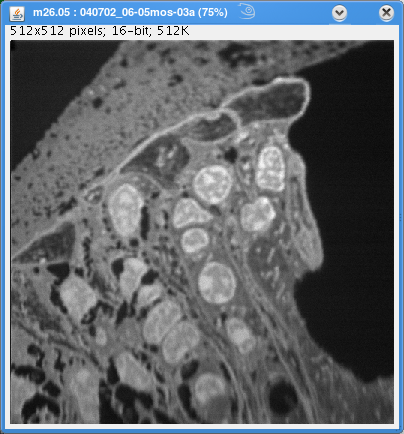
\includegraphics[scale=0.45]{snapshot_cochlea_m26.png}
	}
	\subfigure[mass 27.03,  $^{12}$C$^{15}$N]{
	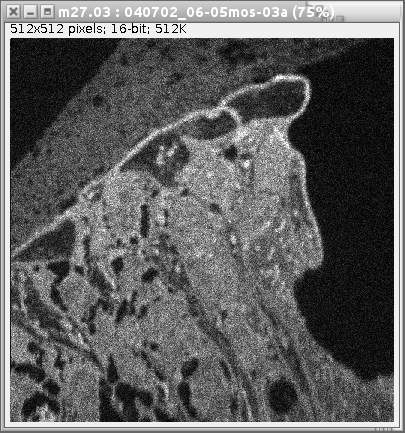
\includegraphics[scale=0.45]{snapshot_cochlea_m27.png}
	}
	\caption{Two different mass images of the same field of view.}
	\end{figure}


\newpage
\section*{Graphical Interface}
	
	The NRIMS Analysis Module window contains 7 tabs:
	\begin{itemize}
	\item \textbf{MIMS Data:} Displays metadata and other information for the current file.
	\item \textbf{Process:} Used to generate ratio images and HSI maps.
	\item \textbf{Contrast:} Controls the contrast and brightness settings for mass, ratio and sum images.
	\item \textbf{Stack Editing:} Used for manipulating the mass images (applying x and y translations, dropping planes, etc).
	\item \textbf{Tomography:} Basic plotting of statistics for whole images or ROIs.
	\item \textbf{Segmentation:} Perform an algorithmic segmentation of an image.
	\item \textbf{MIMS Log:} Displays more header metadata and a record of the user's actions and debug output.
	\end{itemize}
	\vfill
	\begin{figure}[ht]
	\centering
	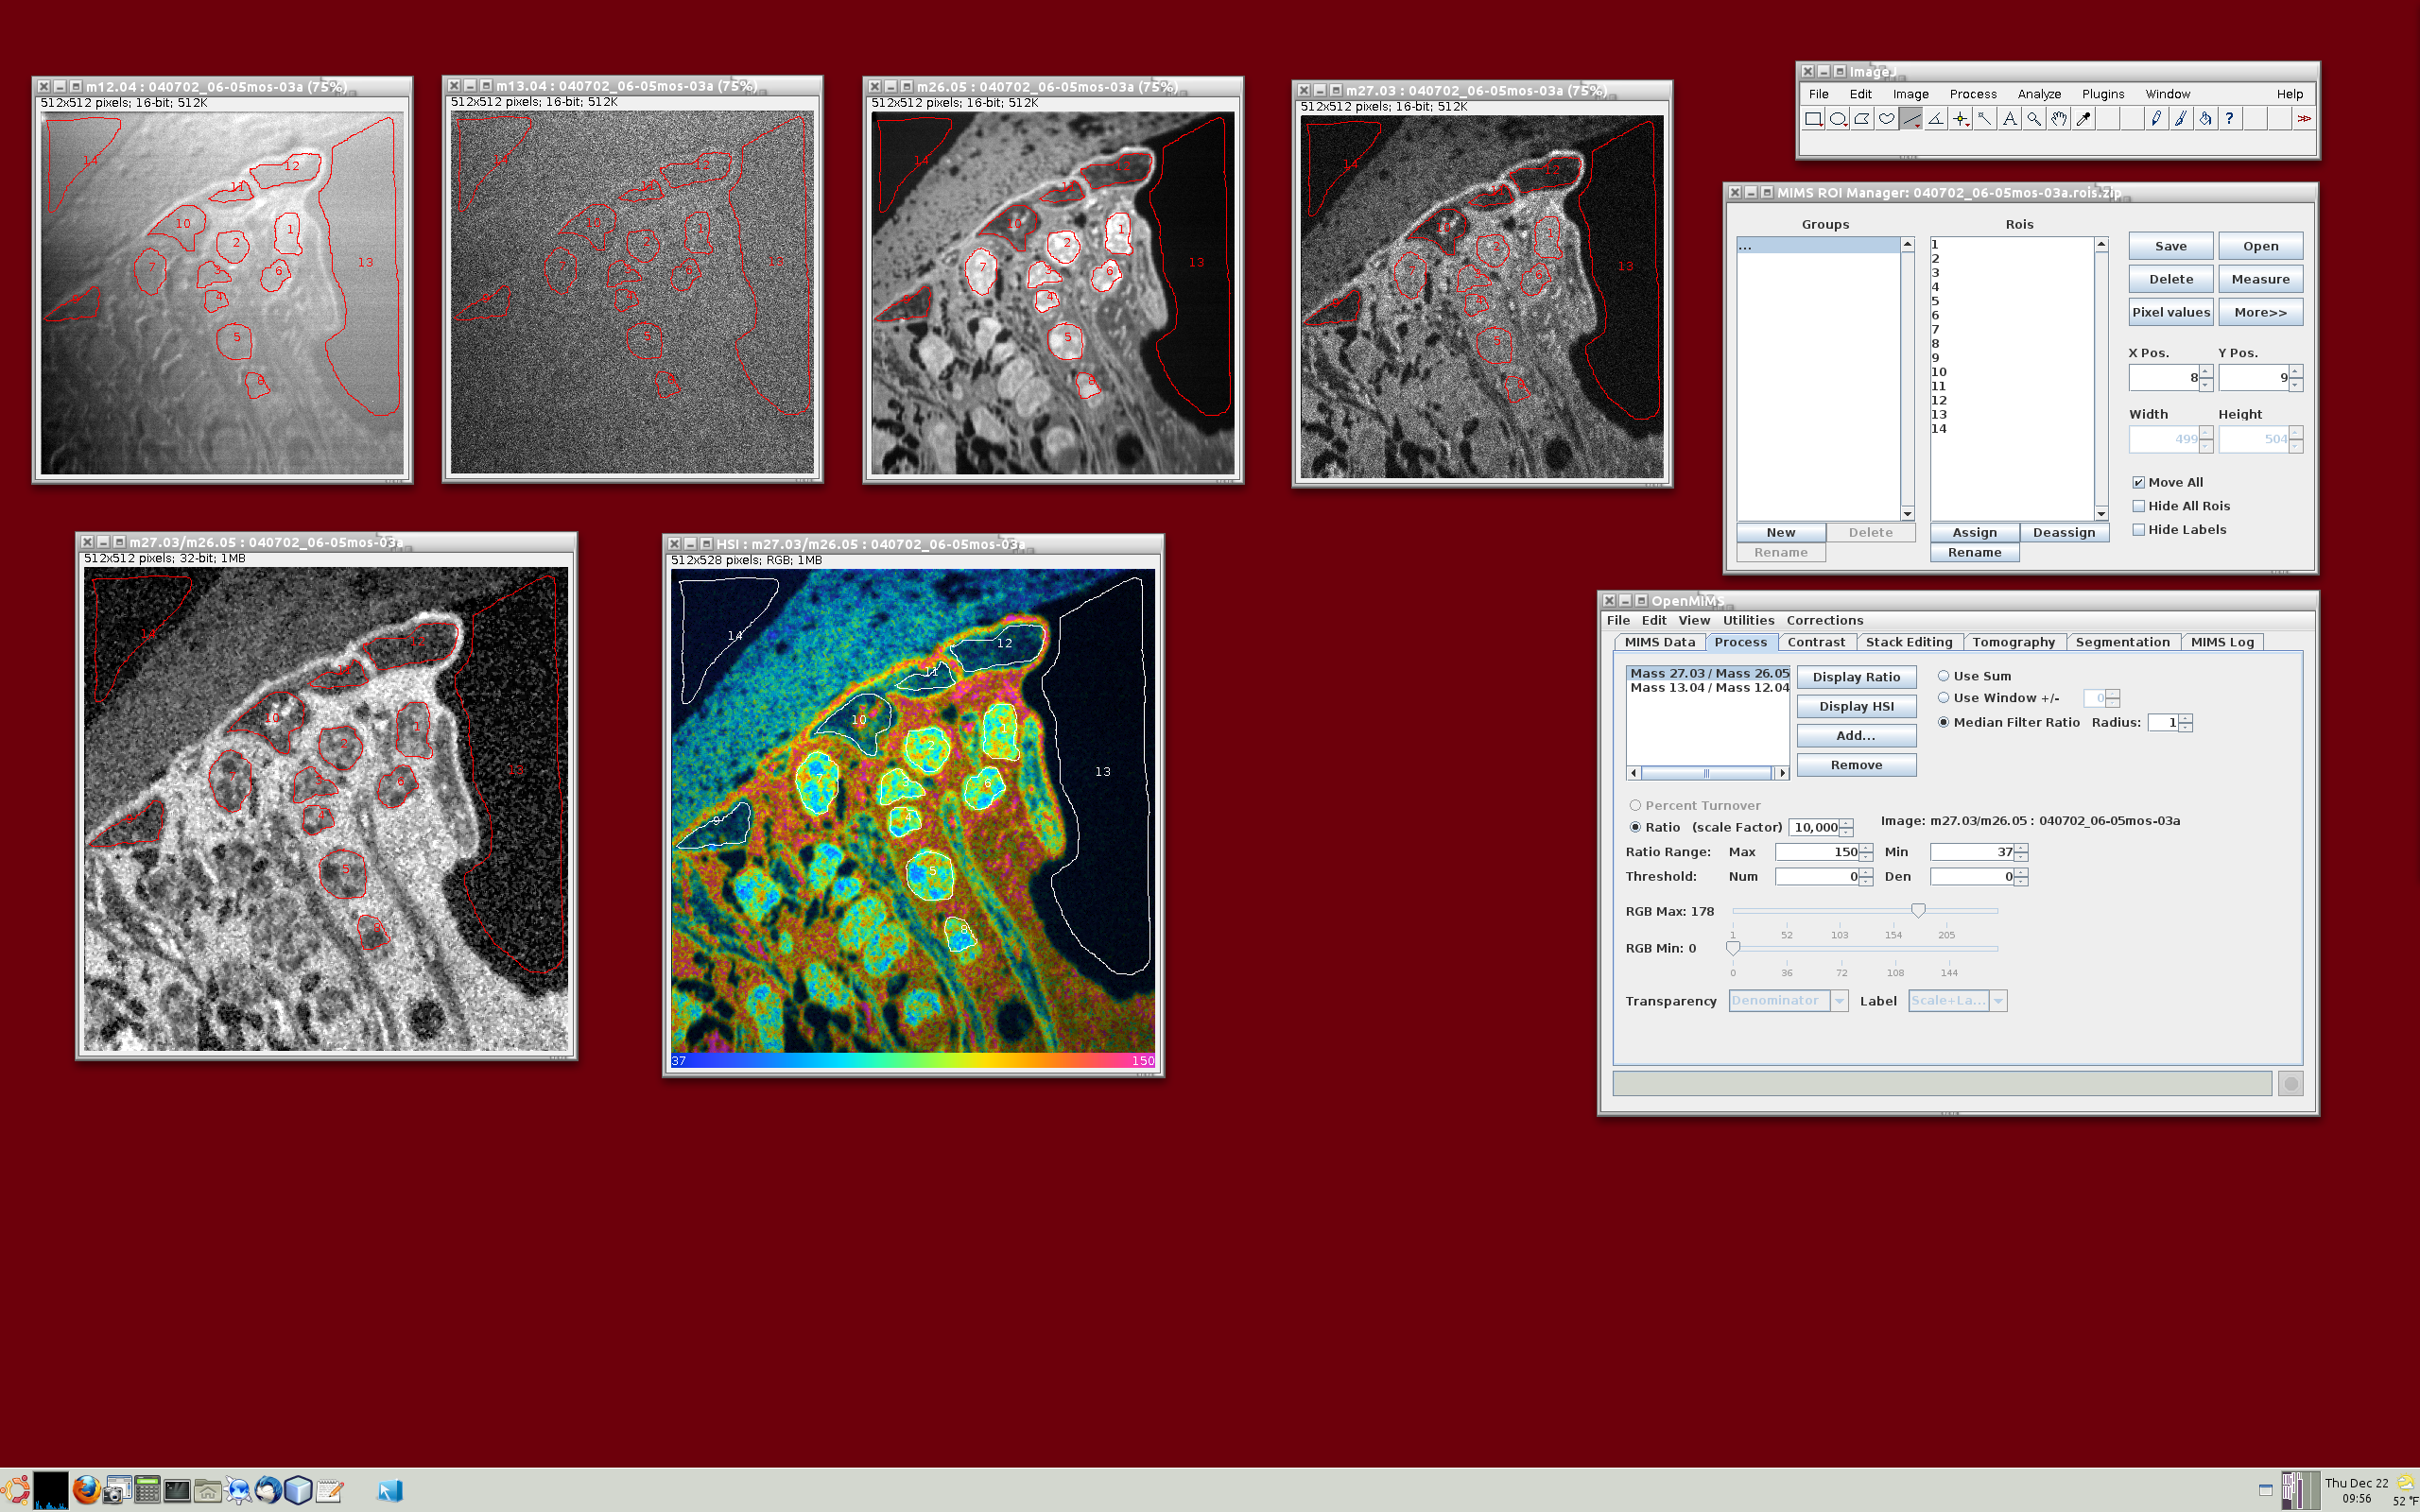
\includegraphics[width=\textwidth]{snapshot_Desktop_3.png}
	\caption{A desktop screenshot of the OpenMIMS application.}
	\end{figure}


\newpage
\section*{MIMS Data:}
	
	\begin{figure}[h]
	\centering
	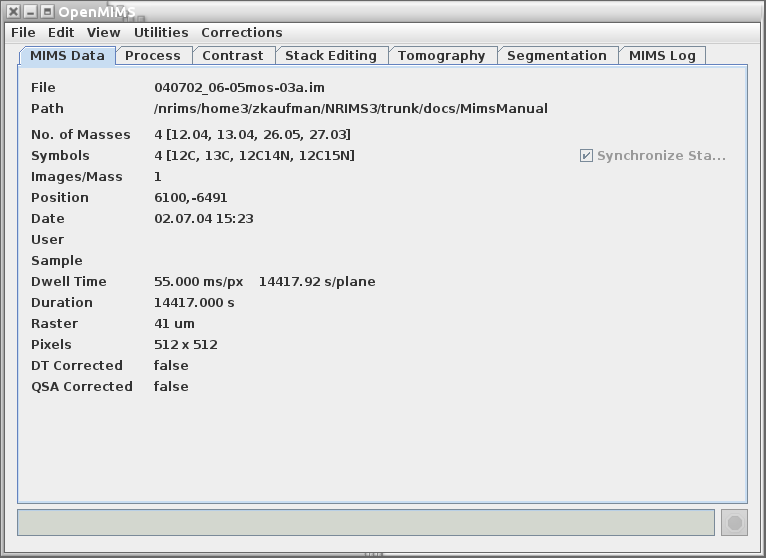
\includegraphics[scale=0.70]{snapshot_MimsData.png}
	\caption{The \textbf{MIMS Data} tab displays file information and meta data.}
	\end{figure}
	
	The \textbf{MIMS Data} tab displays a subset of the image's meta-data
	including the absolute path of the current image, the number of masses 
	and their AMU values, number of planes in the stack, position, date 
	of image, user name, dwell time, duration, raster size and image size. 
	The \textbf{Synchronize Stacks} check box enables updating of all masses 
	simultaneously while scrolling through an image stack. Adjusting the 
	slider (plane selector) at the bottom of any mass automatically selects 
	the same plane for all masses.


\newpage
\section*{Process:}
	
	\begin{figure}[h]
	\centering
	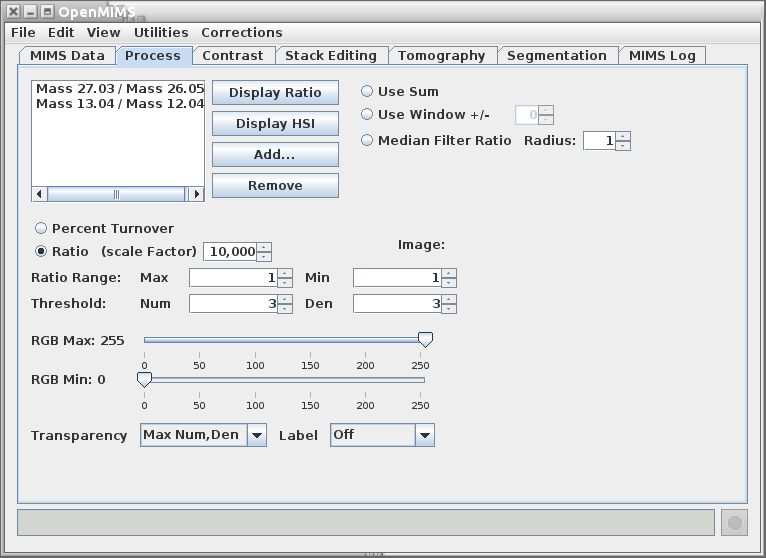
\includegraphics[scale=0.65]{snapshot_Process.png}
	\caption{The \textbf{Process} tab is used to generate ratio and HSI images.}
	\end{figure}

	The \textbf{Process} tab allows the user to generate ratio images and HSI maps. 
	Ratio and HSI images are the result of dividing one mass image by another. Masses that have 
	similar values will automatically show up in list form in the \textbf{Process} tab.
	Others that do not show up by default can be 
	entered manually using the \textbf{Add...} button.
	A ratio image will appear when the user selects one (or more) in the list and 
	clicks \textbf{Display Ratio}. When moving the mouse pointer 
	over the ratio image, the 
	status box along the lower border of the NRIMS Analysis Module window displays 
	the raw numerator and denominator counts as well as the ratio value.

	HSI images are similar to ratio images but are different
	in that they use a combination of the the ratio value of a pixel, the counts of one of 
	the masses for the intensity, and a constant saturation value, to generate pixels in the RGB 
	color space. Clicking the \textbf{Display HSI} will make the selected HSI image appear. An example 
	HSI image is provided in \textbf{APPENDIX A}. When displaying HSI
	images, the user has the option of displaying the actual ratio values 
	(multiplied by the \textbf{Ratio Scale Factor}) or displaying percent turnover by selecting the 
	\textbf{Percent Turnover} radio button. Percent turnover is determined by the naturally occurring ratio
	of that specific isotopic pair along with the maximum achievable ratio based on the experimental protocol.

	The \textbf{Threshold} option sets the minimum number of counts in the numerator and/or 
	denominator. Any pixels below that threshold will be ignored and appear black.
	The \textbf{Ratio Range Min} and \textbf{Max} values determine the range of the colormap
	used to display the image. The \textbf{RGB Min} and \textbf{RGB Max} values determine
	the intensity scale used in the image. The \textbf{Transparency} selects the 
	method for computing the intensity component of the HSI image, and the \textbf{Label} 
	option enables a color scale bar to be become visible. Selecting the \textbf{Use Sum}
	radio button will generate a single HSI (or ratio) image representative of the entire stack. Selecting 
	the \textbf{Use Window} radio button will use the sum of both masses over a sliding window 
	with the specified window size. This can be very useful for finding small features in large image 
	stacks that have low counts. Also, a median filter 
	can be applied to a ratio or HSI image by selecting the \textbf{Median Filter Ratio} 
	radio button.


\newpage
\section*{Contrast:}
	
	\begin{figure}[h]
	\centering
	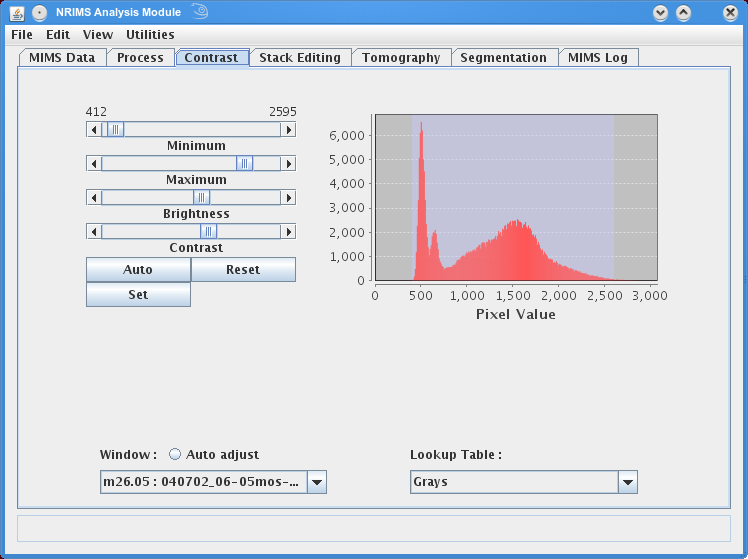
\includegraphics[scale=0.70]{snapshot_MimsContrast.png}
	\caption{The \textbf{Contrast} tab controls and displays contrast settings for mass, ratio and sum images.}
	\end{figure}
	
	The \textbf{Contrast} tab allows the user to control the contrast settings, by adjusting 
	the sliders, for any given mass,
	ratio or sum image (HSI images do not have contrast settings, instead their display
	parameters are controlled using the \textbf{Process} tab).
	It also displays a histogram of intensity values for any of these types of images.
	Clicking on an image brings it into focus and the histogram and
	contrast settings will update to reflect the values of the current image in focus.
	The histogram and contrast settings will also update by selecting the window in the
	combobox located at the bottom of the \textbf{Contrast} tab. All mass, ratio and sum images
	should appear in the combobox.

	If changes to the default contrast settings are made, clicking the \textbf{Reset} button will
	bring those settings back to their default values. Clicking \textbf{Auto} will
	iterate through a set (usually 5 or 6) of contrast settings, eventually returning
	back to default values. The \textbf{Set} button allows the user to input values for min and
	max that are outside the range of those provided by the \textbf{Minimum} 
	and \textbf{Maximum} sliders.

	Mass, ratio and sum images can also be set to \textbf{Auto Adjust} meaning that
	each time a new slice is selected in the stack, new contrast settings are calculated.
	If \textbf{Auto Adjust} is not selected, the contrast settings for the first image
	in the stack are used throughout the stack.

	The user has the additional capability of displaying the image using \textbf{Lookup
	Tables} other than the gray table used by default. There are several options for
	displaying the data and each image can be set independently.


\newpage 
\section*{Stack Editing:}
	
	\begin{figure}[h]
	\centering
	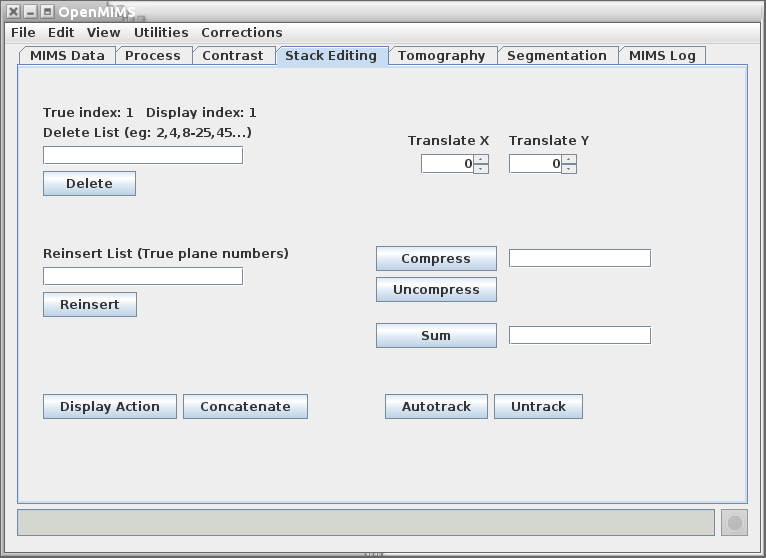
\includegraphics[scale=0.65]{snapshot_MimsStackEditing.png}
	\caption{The \textbf{Stack Editing} tab is used for image manipulation.}
	\end{figure}
	
	The \textbf{Stack Editing} tab is reserved for functions that relate to the editing
	and manipulating of mass images. This includes deleting and reinserting planes,
	applying translation, compressing the image and generating sum images. 
	One important thing to note is that there
	are two indices for an image, both of which are displayed: \textbf{True index} and 
	\textbf{Display index}. The True index of a
	plane in an image never changes, but the Display index depends on what planes have been deleted. For
	example: entering “1-5” and clicking the \textbf{Delete}, then entering “6-10”, 
	and clicking “Delete” will -not- delete the first 10
	planes of an image. Doing that is equivalent to entering “1-5, 11-15” and clicking \textbf{Delete}. 
	The \textbf{Reinsert} button uses the indices of the original data, so entering
	entering “1-5, 11-15” would reinsert the previously deleted planes.
	
	A plane that is currently displayed can be translated using 
	the \textbf{Translate X} or \textbf{Translate Y} spinners, or by
	entering a value those text fields. The image can also be 
	registered automatically by clicking on a specific mass
	to use and then clicking the \textbf{Autotrack} button. 
	This will call the autotrack algorithm 
	which will automatically attempt to determine the best 
	per image translations for a best fit alignment
	throughout the stack. Clicking \textbf{Untrack} will 
	reset all translations to zero.

	The \textbf{Concatenate} button allows another image (or image stack) to be
	prepended or appended to the current image set. The \textbf{Sum} button will 
	generate a sum image from whichever mass image or ratio
	image was most recently clicked. If the field is blank the entire image is summed, 
	or a range of planes can be entered in the textfield (e.g. 1-20). The \textbf{Compress} button 
	compresses the images into blocks of the size entered in the text field. Entering 
	a value of 4 in the field will sum the pixel values in blocks of 4 planes,
	resulting in a stack of images 1/4 the original size. Any
	remaining planes at the end of the stack are summed together into a single block.
	The \textbf{Uncompress} button undoes the compression and restores the image to its original
	state - minus any translations applied and planes deleted.

%	 The \textbf{Display Action} button produces a window which displays
%   current state of the users ``analysis session''. The action window lists 
%   which planes have been dropped, the translation, and the names of all 
%   appended and prepended image files. A sample
%	 action file is shown in Appendix B.


\newpage
\section*{Tomography:}
	
	\begin{figure}[h]
	\centering
	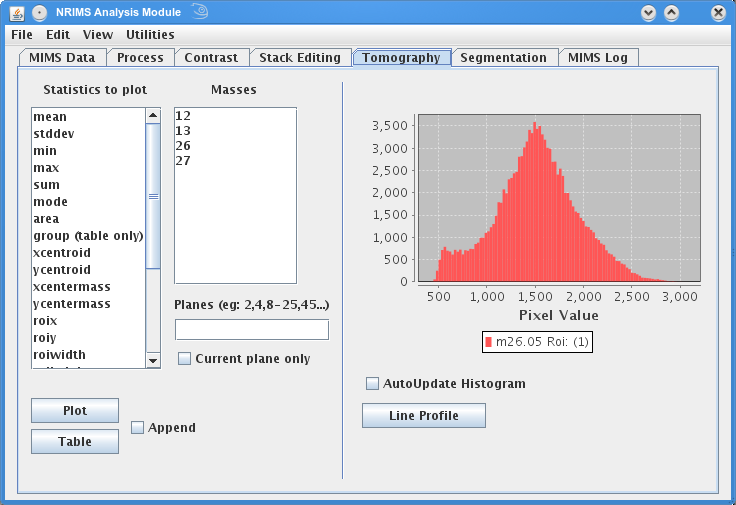
\includegraphics[scale=0.68]{snapshot_MimsTomography.png}
	\caption{The \textbf{Tomography} tab is used to generate plots and tables of ROI statistics.}
	\end{figure}
	
	The \textbf{Tomography} tab allows the user to generate simple line plots or tables
	of ROI statistics through the stack. Simply select a set of ROIs from the 
	\textbf{ROI Manager}, the desired statistics, and the mass, ratio and/or sum  
	images and click \textbf{Plot} or \textbf{Table}.
	The \textbf{Planes} field allows the user to enter which planes are 
	included in the plot (or table). If this field is left blank, all planes will be 
	included. Checking the \textbf{Append} box will append the data to an existing
	plot or table if one exists, otherwise a new one will be created. An example of 
	the type of plot produced can be seen in Figure 8. 
	
   \begin{figure}[h!]
	\centering
	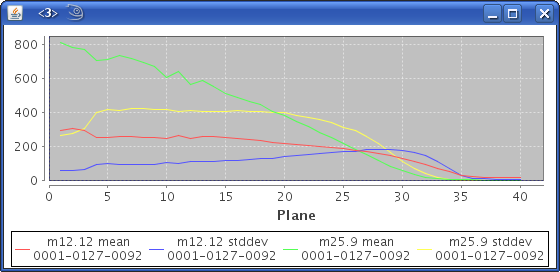
\includegraphics[scale=0.82]{snapshot_TomographyPlot2.png}
	\caption{An example plot of the \textit{mean} and \textit{stdev} statistics for two different masses.}
	\end{figure}

	The table output will vary depending on the type of images for which
	statistics are being generating. Mass and ratio images that are more
	than one plane will output one row of data per plane. In the case of
	sum images and other images that are only one plane, one row of data
	will be produced per ROI. See \textbf{APPENDIX B} for a sample data output table.
	
	The right side of the tab includes a histogram that displays the intensity values for 
	the pixels within a given ROI.
	To set which ROI values are displayed by the histogram, the user only needs to 
	scroll the mouse over the desired ROI. After a ROI has been drawn, it can be moved
	anywhere within the image by either dragging it with the mouse, or using the position
	spinners in the \textbf{ROI Manager}. If the \textbf{Autoupdate Histogram} radio 
	button is selected, the histogram will update as the ROI is being moved by the mouse.
	Otherwise, it updates when the move is complete.

	A line ROI represents a special case because it has no enclosed area, so its values will
	not be represented in the histogram. Instead, the user can select the \textbf{Dynamic
	Profile} button to generate a profile plot of the pixels which the line intersects. An
	example of a mass image with a line ROI and its profile plot is provided below.

	\begin{figure}[h]
	\centering
	\subfigure[]{
	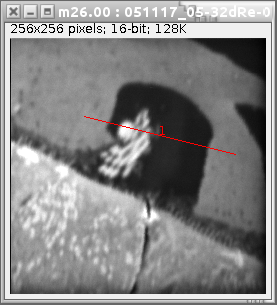
\includegraphics[scale=0.80]{snapshot_LineROI.png}
	}
	\hfill
	\subfigure[]{
	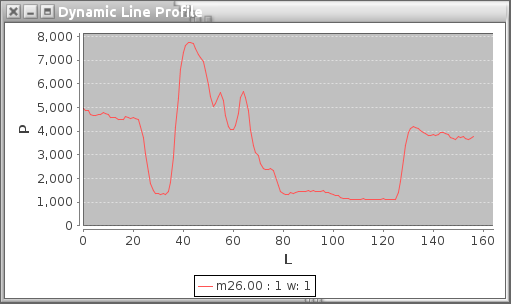
\includegraphics[scale=0.79]{snapshot_ProfilePlot.png}
	}
	\caption{A mass image with a line ROI (a) and its corresponding Profile Plot (b).}
	\end{figure}
	\clearpage

\newpage
\section*{Segmentation:}
	
	\begin{figure}[h]
	\centering
	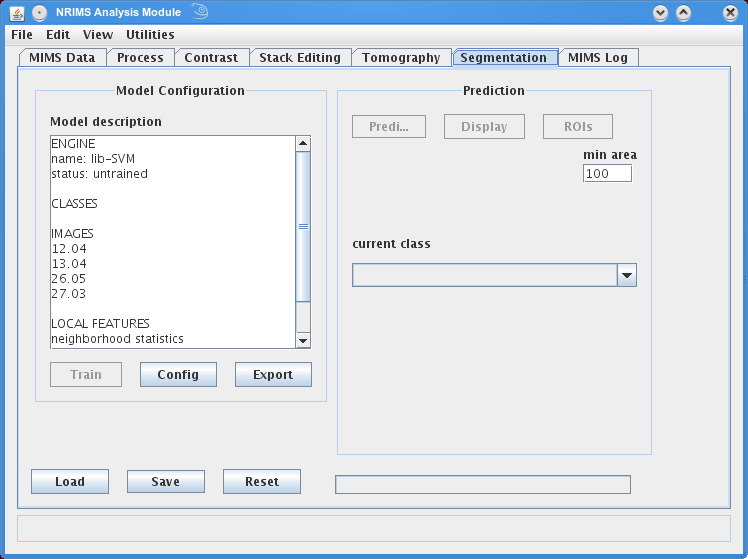
\includegraphics[scale=0.70]{snapshot_MimsSegmentation.png}
	\caption{The \textbf{Segementation} tab.}
	\end{figure}
	The \textbf{Segmentation} tab allows the user to perform an algorithmic segmentation of a MIMS image to automatically generate ROIs for a given image plane. The algorithm used is a support vector machine (SVM) based segmentation that classifies pixels in the image using methods similar to \textit{Fuller et. al.} [1]. A full description of SVMs is outside the scope of this document but will be detailed in a forthcoming paper.  The algorithm can use many values or features to classify a pixel: the value of that pixel in a set of mass or ratio images, the mean and standard deviation in a neighborhood around that pixel, and the gradient around that pixel. Note that the ability to use other features may be added later. To perform a segmentation the user clicks on the \textbf{Config} button and is presented with a window as shown in Figure 10.  The \textbf{Export} button will export the SVM and data if the SVM has been trained using the libSVM format.

	\begin{figure}[h]
	\centering
	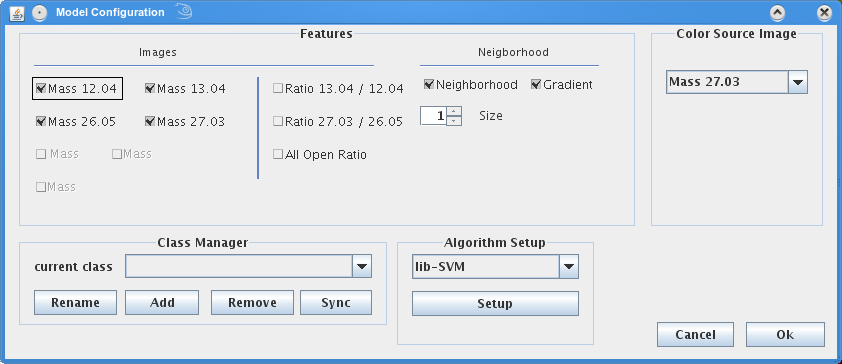
\includegraphics[scale=0.65]{snapshot_Model_Config.png}
	\caption{SVM configuration GUI.}
	\end{figure}

	Here the user may select which mass and ratio images to use for the segmentation 
	(segmentation can not be performed on Sum images).  One can choose whether or not 
	to use the \textbf{Neighborhood} parameters (mean and standard deviation) and the 
	\textbf{Gradient} as features, as well as the size of the neighborhood radius. 
	Some parameters used by the SVM library (in our case libSVM [2]) by clicking the 
	\textbf{Setup} button, specifically the type of kernel to use and the level of 
	cross validation.  We recommend using the radial basis function (\textit{RBF}) 
	as the kernel.  The level of cross validation may be reduced to increase speed 
	at the possible cost of accuracy.

	To train the SVM the user needs to choose at least several ROIs that represent 
	a given class of pixels. First a class is added to the \textbf{Class Manager} 
	by clicking the \textbf{Add} button.  Then the representative ROIs are drawn.  
	Then the \textbf{Sync} button is clicked to sync the ROIs in the \textbf{ROI Manger} 
	to the class in the \textbf{Class Manager}. Finally the users clicks the \textbf{Ok} 
	button to complete the SVM configuration.


\newpage
	The SVM must be trained by clicking the \textbf{Train} button, located below 
	\textbf{Model description} in Figure 11.  It should be noted that the SVM can 
	be saved either before training (saving all parameter settings and training ROIs) 
	or after training (also saving the trained SVM).  The segmentation of the entire 
	image can be performed by clicking \textbf{Predict} and the result of this 
	prediction can be shown by clicking \textbf{Display}. Currently the SVM only 
	segments 2D images. Generating ROIs from the prediction can be done by clicking 
	\textbf{ROIs} which will generate a set of ROIs for each class ignoring groups 
	of pixels of the same class that are below the value in the \textbf{min area} 
	field. An example of a segmentation can be seen in \textbf{APPENDIX C}.

\newpage
\section*{Mims Log:}
	
	\begin{figure}[h]
	\centering
	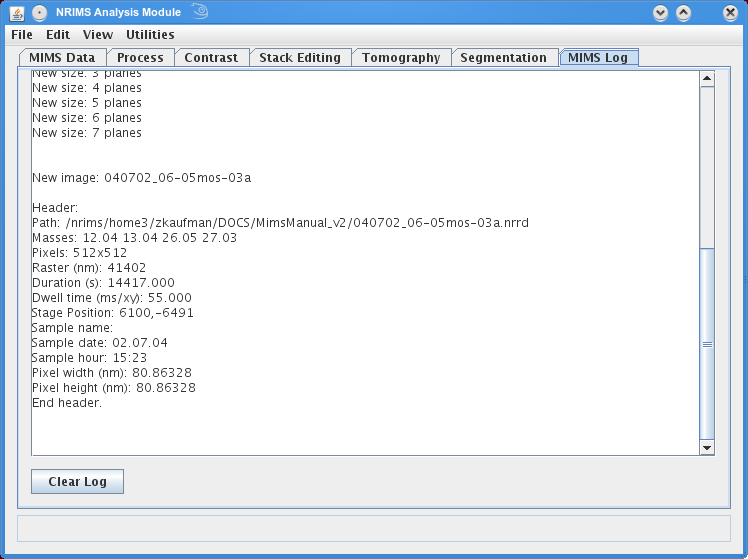
\includegraphics[scale=0.70]{snapshot_MimsLog.png}
	\caption{The \textbf{MIMS Log} tab contains metadata and debug information.}
	\end{figure}
	
	The \textbf{MIMS Log} tab keeps a record of what the user has done: 
	e.g. deleting planes, translating planes, autotracking, etc. Various bits
	of degub data are also displayed on this tab.
	This information is not saved and is most likely of little use to the most users.


\newpage
\section*{ROI Manager:}
\subsection*{Creating Regions of Interest (ROIs)}

	The ROI Manager (see Figure 13) gives the user functionality relating the ROIs
	in a given image. It is comprised of two lists, one labeled \textbf{Groups} and
	one labeled \textbf{Rois}, as well as a panel on the right hand side containing 
	buttons, spinners and checkboxes. 

   To create a ROI, first select the type of ROI to draw by clicking
   one of the corresponding toolbar buttons in ImageJ's main window (any of the five buttons on the left,
   i.e Rectangle, Circular, Polygon.. etc, see the top right window in Figure 2).
   Then place the mouse over the area and drag the mouse while holding the left mouse button down. When the left
   mouse button is released, the corresponding ROI will appear in all image windows
   as well as in the list of ROIs in the ROI manager.
   Clicking on a previously drawn ROI in \textbf{ROI Manager} list will automatically highlight the selected
   ROI in all mass, ratio, sum and HSI images.
   
	\begin{figure}[ht]
	\centering
	\subfigure[Mass image with ROIs,  $^{12}$C$^{14}$N]{
	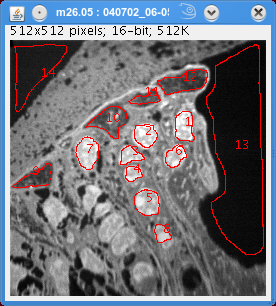
\includegraphics[scale=0.82]{snapshot_m26ROIs.png}
	}
	\hfill
	\subfigure[The ROI Manager]{
	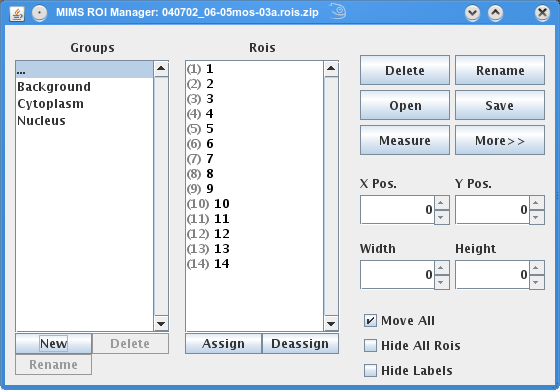
\includegraphics[scale=0.6]{snapshot_ROImanager.png}
	}
	\caption{A mass image with serveral ROIs (a) and the corresponding ROI Manager (b). }
	\end{figure}
	
	The \textbf{Groups} list allows the user to organize ROIs into groups.
   The user can create new groups, delete existing ones, and assign ROIs into groups.
   An ROI can only belong to a single group. Clicking on a group will reduce the \textbf{Rois} 
   list to only those ROIs belonging to that group. Clicking on the elipses group
   (\textbf{...}) will always show all ROIs.

	\textbf{Delete} will delete the selected ROIs in the ROI list.
	If none are selected then it will delete them all, after prompting the user. \textbf{Rename}
	allows the user to rename the ROI from its default name.
	\textbf{Open} will open an ROI file that had been saved from a previous session and overwrites the current list.
	\textbf{Save} will save a single ROI to a file or a group of them to a \textit{.zip} file.
	\textbf{Measure} will open a statistics box that will display statistics for all ROIs for
	the current image. \textbf{Deselect} will deselect any ROIs that have been highlighted. The
	\textbf{More$>>$} button offers the user some more complicated features relating to the 
	combining and splitting ROIs. ROIs can be moved on a pixel by pixel basis using the 
	\textbf{X Pos.} and \textbf{Y Pos.} spinners. ROIs can also be moved by the user by 
	dragging them across the image with the mouse cursor. Adjusting the \textbf{Width} and
	\textbf{Height} spinners will adjust those values but only for rectangular and circular ROIs.

	If the user moves an ROI, it will move for all images in the stack 
	unless the \textbf{Move All} checkbox is unchecked, in which it will 
	only be moved for the current plane. The user can choose to hide all
	ROIs by checking the \textbf{Hide All Rois} checkbox or just hide the labels
	by checking the \textbf{Hide Labels} checkbox.
   

\newpage
\section*{Menu Items}
	\noindent This section provides a brief description of features provided in the menu items
	of the MIMS application
	\begin{figure}[h]
	
\includegraphics[scale=0.60]{snapshot_MenuItems.png}
	\end{figure}
	\begin{description}
	
	\item[\large{File}] \indent                       
	
	\begin{description}
	
	\item[Open MIMS Image:] This menu item will bring up a file chooser that allows the user to select 
	which file should be opened. The plugin can read \textit{.im} files and \textit{.nrrd} files [3] (It 
	can only open the \textit{.nrrd} files that were generated by the plugin). Additionally it can open
	any \textit{.ratio}, \textit{.hsi}, and \textit{.sum} file that was generated by the plugin
	when saving from a previous session.
	
	\item[Save Image:]  This menu item will save whatever modifications have been made to the original
	\textit{.im} file (translations, dropped planes, etc.) into a new binary file with a \textit{.nrrd}
	file extension. The OpenMIMS plugin is capable of reading the both \textit{.im} files and the \textit{.nrrd}
	files that it generates.
	
	\item[Save Session:] This menu item is similar to the \textbf{Save Image} menu item however 
	in this case additional files will be created for each ratio, hsi and sum image that is 
	open at the time of saving. These files can be opened individually at a later date so long
	as the \textit{.nrrd} file that was created with them is stored in the same directory.

	\item[About OpenMIMS:] Displays version and other information related to the OpenMIMS application.
	
	\item[Exit:] Exits the application. ImageJ stays open as well as all opened images.  
	
	\end{description}
	
	\item[\large{Edit}] \indent                       
	
	\begin{description}
	
	\item[Preferences:] Opens a dialog box which allows the user to set customized preferences.
	
	\item[Restore Mims:] This menu item will reset the current image to its
	original state, all translations will be set back to zero and all dropped images will be
	reinserted. Functionally it is the same as reopening the current image. 
	
	\end{description}
	
	\item[\large{View}] \indent                       
	\begin{description}
	
	\item[Tile Windows:] This menu item will take all of the currently open *image* windows
	and rearrange them in a grid on the desktop.
	
	\item[ROI Manager:] This menu item open the ROI Manager. The ROI manager will also
	open whenever a ROI is drawn.
	
	\end{description}
	
	Additional menu items are located here allowing the user to view or hide individual mass images.
	
	\item[\large{Utilities}] \indent                       
	
	\begin{description}
	
	\item[Image Notes:] Opens up a text area that allows user to enter notes regarding an image.
	These notes will be stored with other metadata when saving the file.
	
	\item[Generate Report:] Opens a dialog box which captures the current image and has a text area that
	allows the users to enter notes. When the user clicks OK a .rtf formated report is generated. Subsequent 
	images and notes can be appended to the report. This functionality is useful for recording important
	information while analyzing images.
	
	\item[Sum All Open:] Generates a sum image for all open mass and ratio images. It will not generate
	a sum image for open HSI images. See the \textbf{Process} section to see how
	to generate sum images for HSI images.
	
	\item[Import .im List:] The OpenMIMS application has the ability to read a text file with 
	a list of file names and it will open those image files, appending them to one another. \textit{*NOTE* All
	image files must exist in the same directory as the text file that references them.}
	An example image list file is provided in \textbf{APPENDIX D}.
	
	\item[Capture Current Image:] Selecting this menu item will produce a screen capture of the 
	the last image clicked by the user (whichever image has the current focus). 
	The new image is an RGB image of \textbf{exactly} what is displayed on the screen, 
	including things like ROI outlines.
	
	\item[Batch convert to nrrd:] Allows the user to batch convert a set of .im files into
	.nrrd files. Can also perform tracking of the image while converting.
	
	\item[Export...$>$ Export All Derived (png):] Exports all derived images (ratio, HSI and sum
	images) as .png files.
	
	\item[Close...$>$ Close All Ratio Images:] Closes all currently open ratio images.
	
	\item[Close...$>$ Close All HSI Images:] Closes all currently open HSI images.
	
	\item[Close...$>$ Close All Sum Images:] Closes all currently open sum images.
	
	\item[Generate Stack:] Generates a new ratio or HSI image with independent scrollbars 
	rather than the single plane ratio or HSI images that are generated by default.
	
	\item[Composite:] Selecting this menu item will bring up a dialog which allows the user to quickly create a composite image with up to 4 channels.  Any mass, sum, or ratio image can be used for the Red, Green, Blue, or Grey channels or a channel may be left blank.  Each channel uses a simple color LUT.  The min/max values for each LUT are taken from the underlying images.  For example if the m26 mass image is used for the Red channel that channel will have the same min/max values.  Changing the min/max values (or brightness/contrast) on the Contrast tab for the m26 image will automatically update the Red channel in the composite.
	
	\end{description}
	
	\item[\large{Corrections}] \indent                       
	
	\begin{description}
	
	\item[Apply dead time correction:] Applies a dead time correction to the data. A 44 nanosecond
	correction is applied to the data.
	
	\item[Apply QSA correction:] Applies a QSA correction to the data. Applying the QSA correction
	automatically applies a dead correction.
	
	\end{description}
	\end{description}
	
	\vfill
	
	[1]  Fuller et. al. \textit{Segmentation of Three-dimensional Retinal Image Data.} 
	IEEE Trans. Vis. Comput. Graph. 16(6):1719-1726, 2007.

	[2] libSVM  \textit{http://www.csie.ntu.edu.tw/~cjlin/libsvm/}
	
	[3] http://teem.sourceforge.net/nrrd/

	\clearpage

\newpage
\begin{center}\LARGE{\textbf{APPENDIX A}}\end{center} 
\vfill
\begin{figure}[htp!]
\centering
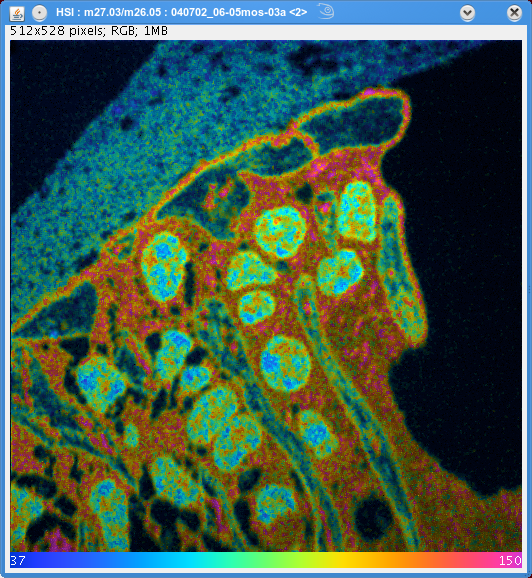
\includegraphics[scale=1.0]{snapshot_HSIimage.png}
\caption{An example of an HSI image.}
\end{figure}
\vfill

\newpage
\begin{center}\LARGE{\textbf{APPENDIX B}}\end{center} 
\vfill
\begin{figure}[h]
\centering
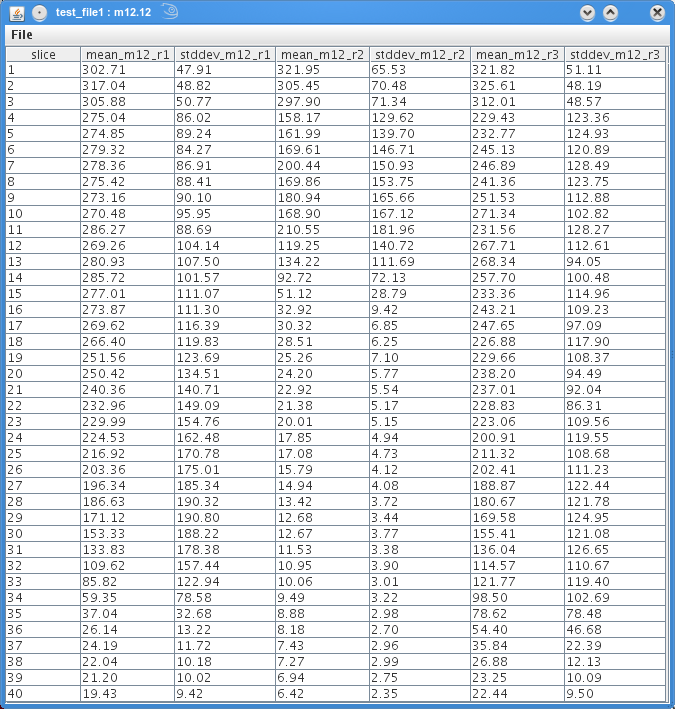
\includegraphics[scale=0.8]{snapshot_Table.png}
\caption{Sample output table showing mean and standard deviation
for a 40 plane image file with three ROIs}
\end{figure}
\vfill

\newpage
\begin{center}\LARGE{\textbf{APPENDIX C}}\end{center} 
\vfill
\begin{figure}[h]
\centering
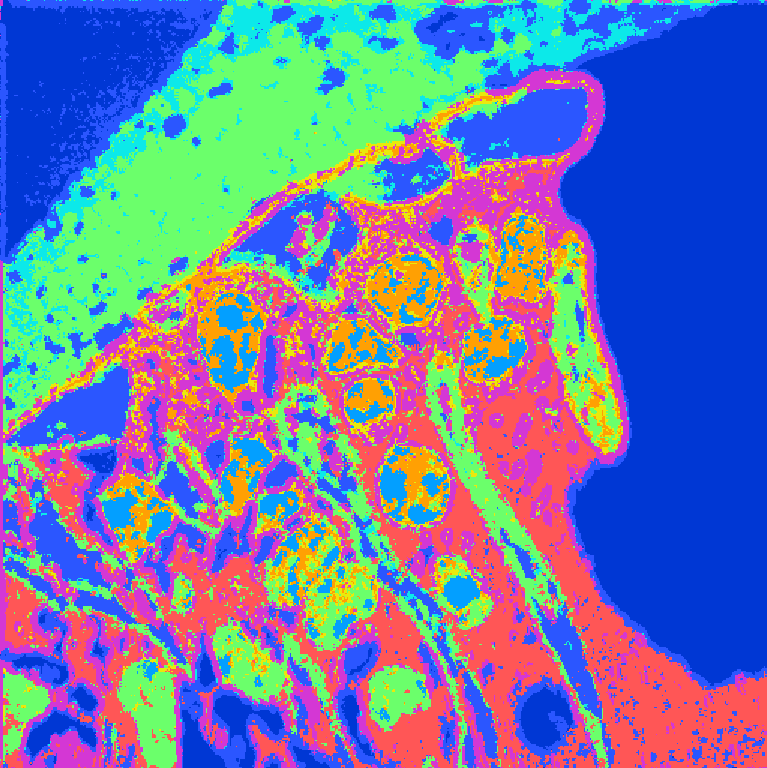
\includegraphics[scale=0.5]{seg_lechene_94p.png}
\caption{A segmented image with 9 classes and no post processing. }
\end{figure}
\vfill


\newpage
\begin{center}\LARGE{\textbf{APPENDIX D}}\end{center} 
\vfill
\begin{figure}[h]
\centering
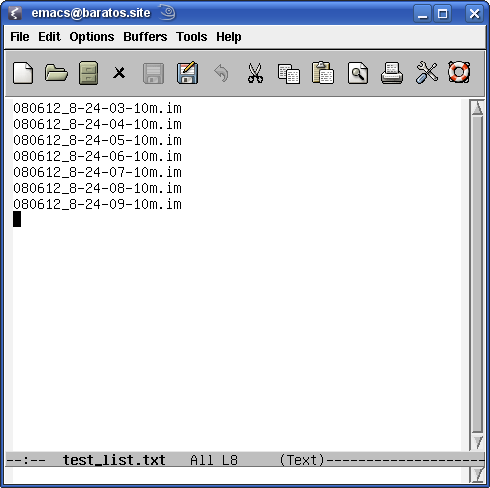
\includegraphics[scale=0.75]{snapshot_ImageList.png}
\caption{A sample image list file.}
\end{figure}
\vfill




\end{document}


